\begin{figure}[htp]
\centering
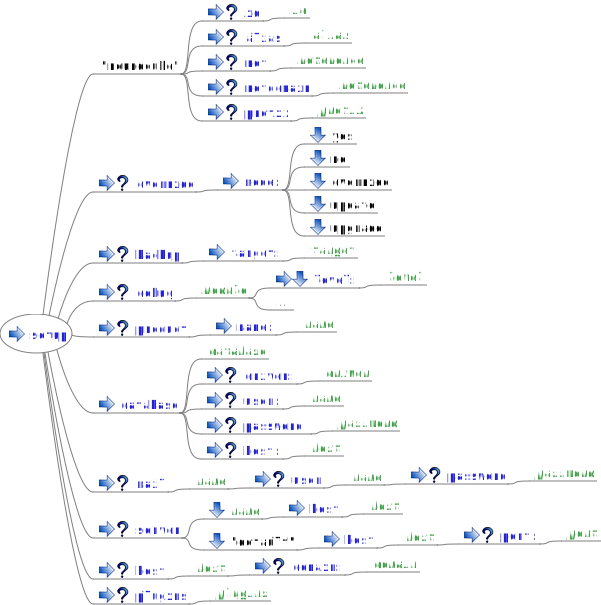
\includegraphics[width=0.8\textwidth]{httpd_setup_roundcube_script}
\label{fig:httpd_setup_roundcube_script}
\caption{Httpd Roundcube Statements}
\end{figure}

%% setup roundcube
\TheStatement[httpd:domain:setup-roundcube]{setup "roundcube"}
\TheStatement*[httpd!domain!setup!roundcube]{setup "roundcube" [, \Arg{id}] [, \Arg{alias}] [, \Arg{ref}] [, \Arg{refdomain}] [, \Arg{prefix}], \{ override backup debug database mail server host \}}

Installs the Roundcube\footnote{\url{http://roundcube.net/}} browser-based
mail client under the domain.

\begin{lstlisting}[style=Java]
httpd {
    domain "test1.com", address: "192.168.0.50", {
        setup "roundcube", alias: "/mail", {
        }
    }
}
\end{lstlisting}

%% override
\TheStatement[httpd:domain:setup-roundcube-override]{override}
\TheStatement*[httpd!domain!setup!roundcube!override]{override mode: \Type{yes} | \Type{no} | \Type{override} | \Type{update} | \Type{upgrade}}

Sets the override mode in case the service is already installed inside
the service prefix.
\begin{asparaitem}
\item \qcode{yes, override} to override the already installed service;
\item \qcode{no} never override the already installed service;
\item \qcode{update} override the already installed service only if the version is the same or newer;
\item \qcode{upgrade} override the already installed service only if the version is newer;
\end{asparaitem}

\begin{lstlisting}[style=Java]
httpd {
    domain "test1.com", address: "192.168.0.50", {
        setup "roundcube", alias: "/mail", {
            override mode: no
        }
    }
}
\end{lstlisting}

%% backup
\TheStatement[httpd:domain:setup-roundcube-backup]{backup}
\TheStatement*[httpd!domain!setup!roundcube!backup]{backup target: \Arg{target}}

Sets the \Arg{target} to where the service backups are stored.

\begin{lstlisting}[style=Java]
httpd {
    domain "test1.com", address: "192.168.0.50", {
        setup "roundcube", alias: "/mail", {
            backup target: "/var/backups"
        }
    }
}
\end{lstlisting}

%% debug
\TheStatement[httpd:domain:setup-roundcube-debug]{debug}
\TheStatement*[httpd!domain!setup!roundcube!debug]{debug \Arg{module}, level: \Arg{level} [, \dots]}

Sets the logging \Arg{level} and other parameters for the debug \Arg{module}.

\begin{lstlisting}[style=Java]
httpd {
    domain "test1.com", address: "192.168.0.50", {
        setup "roundcube", alias: "/mail", {
            debug "roundcube", level: 1
            debug "smtplog", level: 1
            debug "logins", level: 1
            debug "session", level: 1
            debug "sql", level: 1
            debug "imap", level: 1
            debug "ldap", level: 1
            debug "smtp", level: 1
            debug "php", level: 1
        }
    }
}
\end{lstlisting}

%% product
\TheStatement[httpd:domain:setup-roundcube-product]{product}
\TheStatement*[httpd!domain!setup!roundcube!product]{product name: \Arg{name}}

Sets the product \Arg{name} for the service.

\begin{lstlisting}[style=Java]
httpd {
    domain "test1.com", address: "192.168.0.50", {
        setup "roundcube", alias: "/mail", {
            product name: "test1.com mail"
        }
    }
}
\end{lstlisting}

%% database
\TheStatement[httpd:domain:setup-roundcube-database]{database}
\TheStatement*[httpd!domain!setup!roundcube!database]{database \Arg{database} [, driver: \Arg{driver}] [, user: \Arg{user}] [, password: \Arg{password}] [, host: \Arg{host}]}

Sets the database use for the service.
\begin{asparaitem}
\item \Arg{database} the database name;
\item \Arg{driver} optionally, the database driver;
\item \Arg{user} optionally, the database user name;
\item \Arg{password} optionally, the user password;
\item \Arg{host} optionally, the database host;
\end{asparaitem}

\begin{lstlisting}[style=Java]
httpd {
    domain "test1.com", address: "192.168.0.50", {
        setup "roundcube", alias: "/mail", {
            database "roundcubedb", driver: "mysql", user: "userdb", password: "userpassdb", host: "localhost"
        }
    }
}
\end{lstlisting}

%% mail
\TheStatement[httpd:domain:setup-roundcube-mail]{mail}
\TheStatement*[httpd!domain!setup!roundcube!mail]{mail \Arg{name} [, user: \Arg{name}] [, password: \Arg{password}]}

Sets the SMTP mail server settings with the mail server \Arg{name}, optionally 
the SMTP login \Arg{name} and optionally the SMTP login \Arg{password}.

\begin{lstlisting}[style=Java]
httpd {
    domain "test1.com", address: "192.168.0.50", {
        setup "roundcube", alias: "/mail", {
            mail "tls://%h", user: "usersmtp", password: "passwordsmtp"
        }
    }
}
\end{lstlisting}

%% server
\TheStatement[httpd:domain:setup-roundcube-server]{server}
\TheStatement*[httpd!domain!setup!roundcube!server]{server \Arg{name}, host: \Arg{host}}

Adds the IMAP \Arg{host} with the speciefied \Arg{name}.

\begin{lstlisting}[style=Java]
httpd {
    domain "test1.com", address: "192.168.0.50", {
        setup "roundcube", alias: "/server", {
            server "Default Server", host: "mail.example.com"
            server "Webmail Server", host: "webmail.example.com"
        }
    }
}
\end{lstlisting}

%% server "default"
\TheStatement[httpd:domain:setup-roundcube-server-default]{server "default"}
\TheStatement*[httpd!domain!setup!roundcube!server default]{server "default", host: \Arg{host} [, port: \Arg{port}]}

Sets the default IMAP \Arg{host} and optionally the default IMAP host \Arg{port}.

\begin{lstlisting}[style=Java]
httpd {
    domain "test1.com", address: "192.168.0.50", {
        setup "roundcube", alias: "/server", {
            server "default", host: "localhost", port: 143
        }
    }
}
\end{lstlisting}

%% host
\TheStatement[httpd:domain:setup-roundcube-host]{host}
\TheStatement*[httpd!domain!setup!roundcube!host]{host \Arg{host} [, domain: \Arg{domain}]}

Adds the IMAP \Arg{domain} with the speciefied \Arg{host}. If no \Arg{host}
is set, the statement sets the default IMAP domain.

\begin{lstlisting}[style=Java]
httpd {
    domain "test1.com", address: "192.168.0.50", {
        setup "roundcube", alias: "/server", {
            host "example.com", domain: "mail.example.com"
            host "otherdomain.com", domain: "othermail.example.com"
        }
    }
}
\end{lstlisting}

\begin{lstlisting}[style=Java]
httpd {
    domain "test1.com", address: "192.168.0.50", {
        setup "roundcube", alias: "/server", {
            host "example.com"
        }
    }
}
\end{lstlisting}

%% host-default
\TheStatement[httpd:domain:setup-roundcube-host-default]{host}
\TheStatement*[httpd!domain!setup!roundcube!host default]{host \Arg{host}}

Sets the default IMAP \Arg{host}.

\begin{lstlisting}[style=Java]
httpd {
    domain "test1.com", address: "192.168.0.50", {
        setup "roundcube", alias: "/host", {
            host "example.com"
        }
    }
}
\end{lstlisting}

%% plugins
\TheStatement[httpd:domain:setup-roundcube-plugins]{plugins}
\TheStatement*[httpd!domain!setup!roundcube!plugins]{plugins \Arg{plugins}}

Sets the service \Arg{plugins}.

\begin{lstlisting}[style=Java]
httpd {
    domain "test1.com", address: "192.168.0.50", {
        setup "roundcube", alias: "/host", {
            plugins "archive, zipdownload, managesieve"
        }
    }
}
\end{lstlisting}

\subsection{Httpd Roundcube Examples}

\begin{lstlisting}[style=Sscontrol,
label={lst:roundcube_example_script_base},
title={Installs the Roundcube service in the speciefied domain.}]
httpd {
    domain "test1.com", address: "192.168.0.51", {
        setup "roundcube", id: "idroundcube", alias: "roundcube", {
            database "roundcubedb", driver: "mysql", user: "userdb", password: "userpassdb", host: "localhost"
            mail "tls://%h", user: "usersmtp", password: "passwordsmtp"
            backup target: "$tmp/var/backups"
            server "default", port: 981
            server "Default Server", host: "mail.example.com"
            server "Webmail Server", host: "webmail.example.com"
            host "example.com", domain: "mail.example.com"
            host "otherdomain.com", domain: "othermail.example.com"
            plugins "archive, zipdownload, managesieve"
        }
    }
    ssl_domain "test1.com", address: "192.168.0.51", {
        certificate file: certFile, key: certKeyFile
        setup "roundcube", ref: "idroundcube"
    }
}
\end{lstlisting}

\begin{lstlisting}[style=Sscontrol,
label={lst:roundcube_example_script_minimal},
title={Installs the Roundcube service in the speciefied domain with minimal configuration.}]
httpd {
    domain "test1.com", address: "192.168.0.51", {
        setup "roundcube", id: "idroundcube", alias: "roundcubemin", {
            database "roundcubedb", driver: "mysql", user: "userdb", password: "userpassdb"
        }
    }
}
\end{lstlisting}

